%\documentclass[h, xcolor=pst, dvips]{beamer} % presentation normale avec du PSTricks (dvi->ps->pdf)

\documentclass{beamer}

\mode<article> % pour la version 'article'
{
  \usepackage{fullpage}
  \usepackage{hyperref}
}


\mode<presentation> % pour la version 'presentation'
{
  \usetheme{Warsaw} % Warsaw Frankfurt
}


\usepackage[frenchb]{babel}     % specification francaise
\usepackage[latin1]{inputenc}   % entree clavier latin1
% \usepackage[T1]{fontenc}        % sortie

% \usepackage{nameref} % permet d'�crire le nom de la section en cours
% (n�cessite 2 compilations)

\usepackage{graphicx}
\usepackage{tabularx}

\renewcommand{\emph}[1]{\textcolor{red}{\underline{\textit{\textcolor{black}{#1}}}}}

\newcommand{\inclure}[1]{
  \graphicspath{%
    {#1/}%
  }
  \ds{Devoir Surveill�}{
%
}

\nomprenomclasse

\setcounter{numexercice}{0}

%\renewcommand{\tabularx}[1]{>{\centering}m{#1}} 

%\newcommand{\tabularxc}[1]{\tabularx{>{\centering}m{#1}}}

\vressort{3}

\begin{exercice}{Connaissance sur l'atome}%\\
\begin{enumerate}
\item De quoi est compos� un atome ?
\item Que signifie les lettres $A$, $Z$ et $X$ dans la repr�sentation \noyau{X}{Z}{A} ?
\item Comment trouve-t-on le nombre de neutrons d'un atome de l'�l�ment pr�c�dent.
\item Si un atome a $5$ protons, combien-a-t-il d'�lectrons ? Pourquoi ?
\item Qu'est-ce qui caract�rise un �l�ment chimique ?
\item Qu'est-ce qu'un isotope ?
\end{enumerate}
\end{exercice}



\vressort{3}



\begin{exercice}{Composition des atomes}\\
En vous aidant du tableau p�riodique des �l�ments,
compl�ter le tableau suivant :

\medskip

\noindent
%\begin{tabularx}{\textwidth}{|>{\centering}X|>{\centering}X|>{\centering}X|>{\centering}X|>{\centering}X|}
% \begin{tabularx}{\linewidth}{|X|X|X|X|X|}
% \hline
% \emph{nom}       & \emph{symbole}  & \emph{protons} & \emph{neutrons}
% & \emph{nucl�ons} \tbnl
% carbone   & \noyau{C}{6}{14}   &         &          & \rule[-0.5cm]{0cm}{1cm}         \tbnl
% fluor     & \noyau{F}{9}{19}   &         &          & \rule[-0.5cm]{0cm}{1cm}         \tbnl
% sodium    & \noyau{Na}{11}{23} &         &          & \rule[-0.5cm]{0cm}{1cm}         \tbnl
% oxyg�ne   & \noyau{O}{8}{16}   &         &          & \rule[-0.5cm]{0cm}{1cm}         \tbnl
% hydrog�ne &          &         & 0        & \rule[-0.5cm]{0cm}{1cm}         \tbnl
%           & \noyau{Cl}{17}{35} &         &          &  \rule[-0.5cm]{0cm}{1cm}        \tbnl
%           &          & 8       & \rule[-0.5cm]{0cm}{1cm}         & 16       \tbnl
% \end{tabularx}



\begin{tabularx}{\linewidth}{|>{\mystrut}X|X|X|X|X|}
\hline
% multicolumn pour faire dispara�tre le \mystrut
\multicolumn{1}{|X|}{\emph{nom}} & \emph{symbole}  &
\emph{protons} & \emph{neutrons} & \emph{nucl�ons} \tbnl
carbone   & \noyau{C}{6}{14}   &   &   &    \tbnl
fluor     & \noyau{F}{9}{19}   &   &   &    \tbnl
sodium    & \noyau{Na}{11}{23} &   &   &    \tbnl
oxyg�ne   & \noyau{O}{8}{16}   &   &   &    \tbnl
hydrog�ne &                    &   & 0 &    \tbnl
          & \noyau{Cl}{17}{35} &   &   &    \tbnl
          &                    & 8 &   & 16 \tbnl
\end{tabularx}


\end{exercice}


\vressort{3}


\begin{exercice}{Masse d'un atome de carbone 12}\\
Soit le carbone $12$ not� \noyau{C}{6}{12}.
\begin{enumerate}
\item L'�l�ment carbone peut-il avoir $5$ protons ? Pourquoi ?
\item Calculer la masse du noyau d'un atome de carbone $12$
sachant que la masse d'un nucl�on est $m_n = 1,67.10^{-27}~kg$
\item Calculer la masse des �lectrons de l'atome de carbone 12
sachant que la masse d'un �lectron vaut $m_e = 9,1.10^{-31}~kg$
\item Comparer la masse des �lectrons de l'atome � la masse du noyau.
Que concluez-vous ?
\item En d�duire, sans nouveau calcul, la masse de l'atome de carbone
  $12$.
\end{enumerate}
\end{exercice}

\newpage

\vressort{1}

\begin{exercice}{Couches �lectroniques}\\
Dans l'�tat le plus stable de l'atome, appel� �tat fondamental,
les �lectrons occupent successivement les couches,
en commen�ant par celles qui sont les plus proches du noyau : 
d'abord $K$ puis $L$ puis $M$.

Lorsqu'une couche est pleine, ou encore satur�e, on passe � la suivante.

La derni�re couche occup�e est appel�e couche externe.\\
Toutes les autres sont appel�es couches internes.

\medskip

\noindent
%\begin{tabularx}{\textwidth}{|>{\centering}X|>{\centering}X|>{\centering}X|>{\centering}X|}
\begin{tabularx}{\textwidth}{|>{\mystrut}X|X|X|X|}
\hline
\multicolumn{1}{|X|}{\emph{Symbole de la couche}}       & $K$ & $L$ & $M$  \tbnl
\emph{Nombre maximal d'�lectrons} & $2$ & $8$ & $18$ \tbnl
\end{tabularx}

\medskip

Ainsi, par exemple, l'atome de chlore ($Z=17$) a la configuration �lectronique :
$(K)^2(L)^8(M)^{7}$.

\begin{enumerate}
\item Indiquez le nombre d'�lectrons et donnez la configuration des atomes suivants :
  \begin{enumerate}
  \item \noyau{H}{1}{}
  \item \noyau{O}{8}{}
  \item \noyau{C}{6}{}
  \item \noyau{Ne}{10}{}
  \end{enumerate}
\item Parmi les ions ci-desssous, pr�cisez s'il s'agit d'anions ou de cations.
Indiquez le nombre d'�lectrons et donnez la configuration �lectronique
des ions suivants :
  \begin{enumerate}
  \item $Be^{2+}$ ($Z=4$)
  \item $Al^{3+}$ ($Z=13$)
  \item $O^{2-}$ ($Z=8$)
  \item $F^{-}$ ($Z=9$)
  \end{enumerate}
\end{enumerate}

\end{exercice}


\vressort{5}


\begin{exercice}{Charge d'un atome de Zinc}%\\
\begin{enumerate}
\item Combien de protons l'atome de zinc \noyau{Zn}{30}{65} contient-il ?
\item Combien d'�lectrons comporte-t-il ?
\item Calculer la charge totale des protons
sachant qu'un proton a pour charge $e = 1,6.10^{-19}~C$.
\item Calculer la charge totale des �lectrons
sachant qu'un �lectron a pour charge $-e = -1,6.10^{-19}~C$.
\item En d�duire la charge de l'atome de Zinc.
\item Ce r�sultat est-il identique pour tous les atomes ?
\item A l'issue d'une r�action dite d'oxydation, un atome de zinc $Zn$
  se transforme en un ion $Zn^{2+}$.
  \begin{enumerate}
  \item Donnez l'�quation de cette r�action
  (en faisant intervenir un ou plusieurs �lectrons not�s $e^-$).
  \item Indiquez la charge (en coulomb $C$) de cet ion.
  \end{enumerate}
\end{enumerate}
\end{exercice}

\vressort{3}
}

% PSTricks
% \usepackage{pstricks}
% \usepackage{pst-plot} % trac� de fonctions
% \usepackage{pst-circ} % circuit en elec

\newcommand{\actuellement}[1]{%
  \textit{#1}
  % \emph{#1}
}

%\inclure{poste}
\ds{Devoir Surveill�}{
%
}

\nomprenomclasse

\setcounter{numexercice}{0}

%\renewcommand{\tabularx}[1]{>{\centering}m{#1}} 

%\newcommand{\tabularxc}[1]{\tabularx{>{\centering}m{#1}}}

\vressort{3}

\begin{exercice}{Connaissance sur l'atome}%\\
\begin{enumerate}
\item De quoi est compos� un atome ?
\item Que signifie les lettres $A$, $Z$ et $X$ dans la repr�sentation \noyau{X}{Z}{A} ?
\item Comment trouve-t-on le nombre de neutrons d'un atome de l'�l�ment pr�c�dent.
\item Si un atome a $5$ protons, combien-a-t-il d'�lectrons ? Pourquoi ?
\item Qu'est-ce qui caract�rise un �l�ment chimique ?
\item Qu'est-ce qu'un isotope ?
\end{enumerate}
\end{exercice}



\vressort{3}



\begin{exercice}{Composition des atomes}\\
En vous aidant du tableau p�riodique des �l�ments,
compl�ter le tableau suivant :

\medskip

\noindent
%\begin{tabularx}{\textwidth}{|>{\centering}X|>{\centering}X|>{\centering}X|>{\centering}X|>{\centering}X|}
% \begin{tabularx}{\linewidth}{|X|X|X|X|X|}
% \hline
% \emph{nom}       & \emph{symbole}  & \emph{protons} & \emph{neutrons}
% & \emph{nucl�ons} \tbnl
% carbone   & \noyau{C}{6}{14}   &         &          & \rule[-0.5cm]{0cm}{1cm}         \tbnl
% fluor     & \noyau{F}{9}{19}   &         &          & \rule[-0.5cm]{0cm}{1cm}         \tbnl
% sodium    & \noyau{Na}{11}{23} &         &          & \rule[-0.5cm]{0cm}{1cm}         \tbnl
% oxyg�ne   & \noyau{O}{8}{16}   &         &          & \rule[-0.5cm]{0cm}{1cm}         \tbnl
% hydrog�ne &          &         & 0        & \rule[-0.5cm]{0cm}{1cm}         \tbnl
%           & \noyau{Cl}{17}{35} &         &          &  \rule[-0.5cm]{0cm}{1cm}        \tbnl
%           &          & 8       & \rule[-0.5cm]{0cm}{1cm}         & 16       \tbnl
% \end{tabularx}



\begin{tabularx}{\linewidth}{|>{\mystrut}X|X|X|X|X|}
\hline
% multicolumn pour faire dispara�tre le \mystrut
\multicolumn{1}{|X|}{\emph{nom}} & \emph{symbole}  &
\emph{protons} & \emph{neutrons} & \emph{nucl�ons} \tbnl
carbone   & \noyau{C}{6}{14}   &   &   &    \tbnl
fluor     & \noyau{F}{9}{19}   &   &   &    \tbnl
sodium    & \noyau{Na}{11}{23} &   &   &    \tbnl
oxyg�ne   & \noyau{O}{8}{16}   &   &   &    \tbnl
hydrog�ne &                    &   & 0 &    \tbnl
          & \noyau{Cl}{17}{35} &   &   &    \tbnl
          &                    & 8 &   & 16 \tbnl
\end{tabularx}


\end{exercice}


\vressort{3}


\begin{exercice}{Masse d'un atome de carbone 12}\\
Soit le carbone $12$ not� \noyau{C}{6}{12}.
\begin{enumerate}
\item L'�l�ment carbone peut-il avoir $5$ protons ? Pourquoi ?
\item Calculer la masse du noyau d'un atome de carbone $12$
sachant que la masse d'un nucl�on est $m_n = 1,67.10^{-27}~kg$
\item Calculer la masse des �lectrons de l'atome de carbone 12
sachant que la masse d'un �lectron vaut $m_e = 9,1.10^{-31}~kg$
\item Comparer la masse des �lectrons de l'atome � la masse du noyau.
Que concluez-vous ?
\item En d�duire, sans nouveau calcul, la masse de l'atome de carbone
  $12$.
\end{enumerate}
\end{exercice}

\newpage

\vressort{1}

\begin{exercice}{Couches �lectroniques}\\
Dans l'�tat le plus stable de l'atome, appel� �tat fondamental,
les �lectrons occupent successivement les couches,
en commen�ant par celles qui sont les plus proches du noyau : 
d'abord $K$ puis $L$ puis $M$.

Lorsqu'une couche est pleine, ou encore satur�e, on passe � la suivante.

La derni�re couche occup�e est appel�e couche externe.\\
Toutes les autres sont appel�es couches internes.

\medskip

\noindent
%\begin{tabularx}{\textwidth}{|>{\centering}X|>{\centering}X|>{\centering}X|>{\centering}X|}
\begin{tabularx}{\textwidth}{|>{\mystrut}X|X|X|X|}
\hline
\multicolumn{1}{|X|}{\emph{Symbole de la couche}}       & $K$ & $L$ & $M$  \tbnl
\emph{Nombre maximal d'�lectrons} & $2$ & $8$ & $18$ \tbnl
\end{tabularx}

\medskip

Ainsi, par exemple, l'atome de chlore ($Z=17$) a la configuration �lectronique :
$(K)^2(L)^8(M)^{7}$.

\begin{enumerate}
\item Indiquez le nombre d'�lectrons et donnez la configuration des atomes suivants :
  \begin{enumerate}
  \item \noyau{H}{1}{}
  \item \noyau{O}{8}{}
  \item \noyau{C}{6}{}
  \item \noyau{Ne}{10}{}
  \end{enumerate}
\item Parmi les ions ci-desssous, pr�cisez s'il s'agit d'anions ou de cations.
Indiquez le nombre d'�lectrons et donnez la configuration �lectronique
des ions suivants :
  \begin{enumerate}
  \item $Be^{2+}$ ($Z=4$)
  \item $Al^{3+}$ ($Z=13$)
  \item $O^{2-}$ ($Z=8$)
  \item $F^{-}$ ($Z=9$)
  \end{enumerate}
\end{enumerate}

\end{exercice}


\vressort{5}


\begin{exercice}{Charge d'un atome de Zinc}%\\
\begin{enumerate}
\item Combien de protons l'atome de zinc \noyau{Zn}{30}{65} contient-il ?
\item Combien d'�lectrons comporte-t-il ?
\item Calculer la charge totale des protons
sachant qu'un proton a pour charge $e = 1,6.10^{-19}~C$.
\item Calculer la charge totale des �lectrons
sachant qu'un �lectron a pour charge $-e = -1,6.10^{-19}~C$.
\item En d�duire la charge de l'atome de Zinc.
\item Ce r�sultat est-il identique pour tous les atomes ?
\item A l'issue d'une r�action dite d'oxydation, un atome de zinc $Zn$
  se transforme en un ion $Zn^{2+}$.
  \begin{enumerate}
  \item Donnez l'�quation de cette r�action
  (en faisant intervenir un ou plusieurs �lectrons not�s $e^-$).
  \item Indiquez la charge (en coulomb $C$) de cet ion.
  \end{enumerate}
\end{enumerate}
\end{exercice}

\vressort{3} % poste

\title{\poste}
%\title{Titre}

\author{S�bastien \textsc{CELLES}}

\institute{Professeur agr�g� de Sciences Physiques - Physique Appliqu�e}

\date{Mercredi 25 Janvier 2006 - 14h30}
% \date{\today}
% \subject{...}

\begin{document}

\frame{
  % \maketitle
  \titlepage
}


\frame
{
  \tableofcontents
}


\presposte % presentation poste

%\frame{
%  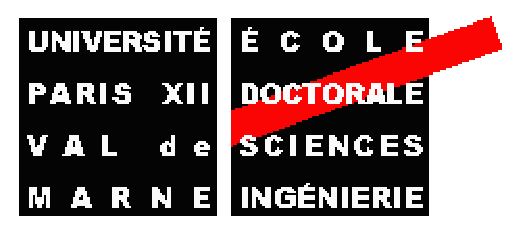
\includegraphics[width=3cm]{logo.gif.eps}
%}

% parcours scolaire




% enseignement
\section{Parcours au sein de l'\'Education Nationale}

\frame{
  \frametitle{Mon parcours au sein de l'\'Education Nationale}

  % \pause

  \begin{itemize}
  \item Professeur stagiaire (2002)
    \begin{itemize}
    \item Physique Chimie en 5$^{\mbox{i\`eme}}$,
      4$^{\mbox{i\`eme}}$\\
      (Coll�ge Jules Vernes - DEVILLE-LES-ROUEN)\\
      Stage en situation

      % \pause

    \item Physique Appliqu�e en 1$^{\mbox{i\`ere}}$ et Terminale \'Electronique\\
      (Lyc�e Marcel SEMBAT - SOTTEVILLE-LES-ROUEN)\\
      Stage de pratique accompagn�e
    
    \end{itemize}
  \end{itemize}
}

\frame{
  \frametitle{Mon parcours au sein de l'\'Education Nationale (suite)}
  

  \begin{itemize}
  \item Titulaire en Zone de Remplacement (TZR) dans le
    d�partement de la Haute-Vienne (2003)
    \begin{itemize}

    \item Classes Pr�paratoires aux Grandes \'Ecoles\\
      \small (Math. Sup. PCSI - Lyc�e Gay Lussac - LIMOGES)
      
      % \pause

      \normalsize

    \item Physique Industrielle en BTS CIRA\\
      \small (Lyc�e Raoul DAUTRY - LIMOGES)
      
      % \pause

      \normalsize
    \item Physique Appliqu�e en lyc�e technologique\\
      1$^{\mbox{i\`ere}}$ \'Electrotechnique,
      Terminale G�nie M�canique\\ \small
      (Lyc�e TURGOT - LIMOGES)
      
      % \pause

      \normalsize
      
    \item Physique Chimie en lyc�e g�n�ral\\ \small
      1$^{\mbox{i\`ere}}$ Scientifique,
      1$^{\mbox{i\`ere}}$ STL C, %Sciences et Techniques de Laboratoire
      Terminale STL Biochimie,
      \actuellement{Seconde Tronc commun et option PCL}\\
      (Lyc�e Raoul DAUTRY - LIMOGES)
      
      \normalsize   
      
    \end{itemize}
  \end{itemize}
}

\frame{
  \frametitle{Autres activit�s au sein de l'\'Education Nationale}

  \begin{itemize}
  \item Formation informatique pour les enseignants
    et les personnels de laboratoire\\
    \begin{itemize}
    \item Notions sur les r�seaux (classe de r�seau, adresse IP)
    \item Notions sur Windows (installation, s�curit�, partage...)
    \item Notions sur le web (aspirer un site, publier un site...)
    \item Quelques applications en milieu scolaire (VNC)
    \item Introduction � quelques logiciels libres
      \begin{itemize}
      \item OpenOffice.org
      \item GIMP
      \end{itemize}
    \end{itemize}
  \end{itemize}
\begin{center}
\url{http://www.celles.net/wikini/wakka.php?wiki=}\\
\url{InfoDautryFormation}
\end{center}
}

\frame{
  \frametitle{Autres activit�s au sein de l'\'Education Nationale}

  \begin{itemize}
  \item Formation informatique pour les enseignants
    et les personnels de laboratoire\\
    \begin{itemize}
    \item Notions sur les r�seaux (classe de r�seau, adresse IP)
    \item Notions sur Windows (installation, s�curit�, partage...)
    \item Notions sur le web (aspirer un site, publier un site...)
    \item Quelques applications en milieu scolaire (VNC)
    \end{itemize}
  \end{itemize}
\begin{center}
\url{http://www.celles.net/wikini/wakka.php?wiki=}\\
\url{InfoDautryFormation}
\end{center}
}

\frame{
  \frametitle{Autres activit�s au sein de l'\'Education Nationale}

  \begin{itemize}
  \item Syst�me de suivi des cours par internet pour une �l�ve hospitalis�e.
    
    \begin{itemize}
    \item Mise en place de SPIP
    \item Formation des �l�ves � l'utilisation en tant que r�dacteur
    \end{itemize}
  \end{itemize}
 
\begin{center}
\url{http://lyc-dautry-87.ovh.org}\\
\end{center}
}

\frame{
  \frametitle{Autres activit�s au sein de l'\'Education Nationale}
  \begin{itemize}
  \item Missions au Centre R�gional de Documentation P�dagogique (LIMOGES)
    \begin{itemize}
    \item R�alisation de maquettes et de documents
      sur les �nergies renouvelables
      \begin{itemize}
      \item \'Energie solaire thermique
      \item \'Energie solaire photovolta�que
      \item \'Energie �olienne
      \item \'Energie hydro�lectrique
      \end{itemize}
    \item R�alisation de documents pour divers mat�riels
      \begin{itemize}
      \item \'Etude des ondes sonores
      \item Mini syst�me d'EXAO
      %\item Mini GBF
      \end{itemize}
    \end{itemize}
  \end{itemize}
\begin{center}
\url{http://www.celles.net/wikini/wakka.php?wiki=}\\
\url{CRDP}
\end{center}
}


\section{En quoi mon parcours est-il adapt� � ce poste ?}

\frame{
  \frametitle{\insertsectionhead}

  \vspace{\stretch{5}}

  \begin{center}
    \begin{Huge}
      En quoi mon parcours convient-il � ce poste ?
    \end{Huge}
  \end{center}
  

  \vspace{\stretch{5}}
}

% info g�n�rale

% langage C
\subsection{Informatique g�n�rale (langage C)}

\frame{
  \frametitle{\insertsubsectionhead}
  %\frametitle{Informatique g�n�rale (langage C)}

  % \pause
  
  \begin{itemize}
  \item Programmation en langage C en ma�trise EEA � l'Universit� Paul
    Sabatier - TOULOUSE III

    % \pause
    
  \item Lecture du livre langage C de \textsc{KERNIGHAN} et
    \textsc{RICHIE}
    
    % \pause
    
  \item Connaissance des outils GNU Make et des Autotools (autoconf, automake)
    
  \end{itemize}
}

% info indus (microcontroleurs)
\subsection{Informatique industrielle (microcontr�leurs)}

\frame{
  \frametitle{\insertsubsectionhead}

  % \pause

  \begin{itemize}
  \item Programmation de microcontr�leurs SAB Siemens C167\\ en langage C
    % \pause
    \begin{itemize}
    \item D�veloppement dans un environnement GNU/Linux
      % \pause
    \item D�veloppement avec GNU Emacs
      % \pause
    \item R�alisation d'un syst�me de distribution de carburant avec
      carte magn�tique (utilisation des interruptions pour la
      lecture de la carte, utilisation des listes cha�n�es pour la
      base de clients, ...)

    \end{itemize}
    
    % \pause

  \item Lectures sur la programmation en assembleur de PIC 16F
    %(cours de \textsc{BIGONOFF})

    % \pause

  \item Programmation en langage C des
    microcontr�leurs ATMEL AVR (ATmega8 et 16) - projets Liberlab, Arduino, OpenChrono
    
    %(articles de GNU/Linux Magazine France, documentation de gcc-avr, projet OpenChrono)

    
  \end{itemize}  

}

% r�seau
\subsection{R�seaux locaux}

\frame{
  \frametitle{\insertsubsectionhead}
  %\frametitle{R�seaux locaux}

  % \pause


  \begin{itemize}
  \item Connaissance du mod�le OSI
    
    % \pause

  \item Lecture : les r�seaux, Guy \textsc{PUJOLLE}
    
    % \pause

  \item R�alisation d'un r�seau personnel
    % \pause
    \begin{itemize}
    \item routeur/firewall sous GNU/Linux IPCop
      % \begin{itemize}
      % \end{itemize}
      % \pause
    \item serveur sous GNU/Linux Debian
      % \pause
      \begin{itemize}
      \item Secure Copy scp par SSH
      \item VNC dans tunnel SSH, export display
      \item Samba
      \item NFS
      \item ...
      \end{itemize}
      % \pause
    \item 2 postes clients
    \end{itemize}
    % \pause
  \item Pratique du routage avec les r�gles iptables sous Linux
  \end{itemize}

  
}


% serveurs
\subsection{Serveurs (web, base de donn�es)}

\frame{
  \frametitle{\insertsubsectionhead}

  % \pause

  \begin{itemize}
  \item Utilisation du serveur web Apache
    % \pause
  \item Langage de scripts PHP avec base de donn�es MySQL
    % \pause
  \item Administration base de donn�es MySQL avec PhpMyAdmin
  \end{itemize}
}

% telecom
\subsection{T�l�communications}

\frame{
  \frametitle{\insertsubsectionhead}
  %\frametitle{T�l�communications}

  % \pause

  \begin{itemize}
  \item Micro-ondes (lignes, guides, propagation, param�tres S, abaque de Smith)
    % \pause
  \item Traitement du signal
    % \pause
  \item Transmission en bande de base
    % \pause
  \item Modulations analogiques (AM, BLU, FM)
    % \pause
  \item Modulations num�riques (ASK,PSK, FSK)
  \end{itemize}
}

% unix linux
\subsection{Unix - Linux}

\frame{
  \frametitle{\insertsubsectionhead}
  %\frametitle{Unix - Linux}

  % \pause

%\begin{center}
%\emph{Utilisation courante des syst�mes Unix et/ou GNU/Linux}
%\end{center}

    % \pause
    \begin{itemize}
    \item Utilisation courante des syst�mes Unix et/ou GNU/Linux
    \item Arborescence, fichiers, liens, droits,
      % \pause
    \item Processus, signaux
      % \pause
    \item Shell : GNU BASH
      % \pause
    \end{itemize}
}


% logiciels libres
\subsection{Logiciels libres}
\frame{
  \frametitle{\insertsubsectionhead}

%  \begin{center}
%    \emph{Go�t pour les logiciels libres}
%  \end{center}

    \begin{itemize}
      
      % \pause
      
    \item Participation � certains projets libres (rapport de bugs
      essentiellement)

      % \pause
      
    \item Cela m'a permis de mieux connaitre les outils (Bugzilla,
      CVS ou Subversion) utilis�s dans ce mode de d�veloppement
    \end{itemize}
    
    % \pause
}


\subsection{Informatique}
\frame{
  \frametitle{\insertsubsectionhead}

  % \begin{center}
  %   \emph{Go�t pour les logiciels libres}
  % \end{center}
  
  \begin{itemize}
  \item Outils de bureautique (Office ou OpenOffice)
  \item Connaissance du d�veloppement web : HTML, CSS, JavaScript, PHP
  \item Connaissance des outils modernes du Web (Content Management
    System comme SPIP, Wiki, Forum...)
    
    % \pause
    
  \item \'Edition scientifique et technique avec \LaTeX
    
    % \pause
    
  \item Connaissance (plus ou moins approfondie) de diff�rents
    langages : Java, C, C++, Python, Ada
  
  \item Documentation de code avec Doxygen
    
    % \pause
    
  \end{itemize}
}



% conclusion
\conclusion

% \frame{
%   \frametitle{\insertsubsectionhead (suite)}

%   \begin{itemize}
%   \item Un envie de 
%   \end{itemize}

% }



\end{document}